\documentclass[submit]{harvardml}

\course{CS181-S21}
\assignment{Assignment \#1}
\duedate{7:59pm ET, February 4, 2021} 
\collaborators{Jonathan Lu, Viet Vu}
\name{Aakash Mishra}

\usepackage[OT1]{fontenc}
\usepackage[colorlinks,citecolor=blue,urlcolor=blue]{hyperref}
\usepackage[many]{tcolorbox}
\usepackage[pdftex]{graphicx}
\usepackage{subcaption}
\usepackage{graphicx}
\usepackage{caption}
\usepackage{fullpage}
\usepackage{soul}
\usepackage{amsmath}
\usepackage{amssymb}
\usepackage{color}
\usepackage{todonotes}
\usepackage{listings}
\usepackage{common}
\usepackage{framed}

\usepackage[mmddyyyy,hhmmss]{datetime}

\definecolor{verbgray}{gray}{0.9}

\lstnewenvironment{csv}{
  \lstset{backgroundcolor=\color{verbgray},
  frame=single,
  framerule=0pt,
  basicstyle=\ttfamily,
  columns=fullflexible}}{}
 

\begin{document}
\begin{center}
{\Large Homework 1: Regression}\\
\end{center}

\subsection*{Introduction}
This homework is on different forms of linear regression and focuses
on loss functions, optimizers, and regularization. Linear regression
will be one of the few models that we see that has an analytical
solution.  These problems focus on deriving these solutions and
exploring their properties.

If you find that you are having trouble with the first couple
problems, we recommend going over the fundamentals of linear algebra
and matrix calculus (see links on website).  The relevant parts of the
\href{https://github.com/harvard-ml-courses/cs181-textbook/blob/master/Textbook.pdf}{cs181-textbook notes are Sections 2.1 - 2.7}.  We strongly recommend
reading the textbook before beginning the homework.

    We also encourage you to first read the \href{http://users.isr.ist.utl.pt/~wurmd/Livros/school/Bishop\%20-\%20Pattern\%20Recognition\%20And\%20Machine\%20Learning\%20-\%20Springer\%20\%202006.pdf}{Bishop textbook}, particularly:
Section 2.3 (Properties of Gaussian Distributions), Section 3.1
(Linear Basis Regression), and Section 3.3 (Bayesian Linear
Regression). (Note that our notation is slightly different but the
underlying mathematics remains the same!).

\textbf{Please type your solutions after the corresponding problems using this
\LaTeX\ template, and start each problem on a new page.} You may find
the following introductory resources on \LaTeX\ useful: 
\href{http://www.mjdenny.com/workshops/LaTeX_Intro.pdf}{\LaTeX\ Basics} 
and \href{https://www.overleaf.com/learn/latex/Free_online_introduction_to_LaTeX_(part_1)}{\LaTeX\ tutorial with exercises in Overleaf}

Homeworks will be submitted through Gradescope. You will be added to
the course Gradescope once you join the course Canvas page. If you
haven't received an invitation, contact the course staff through Ed.

\textbf{Please submit the writeup PDF to the Gradescope assignment
  `HW1'.} Remember to assign pages for each question.

\textbf{Please submit your \LaTeX file and code files to the
  Gradescope assignment `HW1 - Supplemental'.} Your files should be
named in the same way as we provide them in the repository,
e.g. \texttt{T1\_P1.py}, etc.


%%%%%%%%%%%%%%%%%%%%%%%%%%%%%%%%%%%%%%%%%%%%%
% Problem 1
%%%%%%%%%%%%%%%%%%%%%%%%%%%%%%%%%%%%%%%%%%%%%


\begin{problem}[Optimizing a Kernel, 15pts]

Kernel-based regression techniques are similar to nearest-neighbor
regressors: rather than fit a parametric model, they predict values
for new data points by interpolating values from existing points in
the training set.  In this problem, we will consider a kernel-based
regressor of the form:
\begin{equation*}
  f(x^*) = \frac{ \sum_{n} K(x_n,x^*) y_n  }{ \sum_{n} K(x_n,x^*) } 
\end{equation*}
where $(x_n,y_n)$ are the training data points, and $K(x,x')$ is a
kernel function that defines the similarity between two inputs $x$ and
$x'$. Assume that each $x_i$ is represented as a column vector, i.e. a
$D$ by 1 vector where $D$ is the number of features for each data
point. A popular choice of kernel is a function that decays as the
distance between the two points increases, such as
\begin{equation*}
  K(x,x') = \exp(-||x-x'||^2_2) = \exp(-(x-x')^T (x-x') ) 
\end{equation*} 
However, the squared Euclidean distance $||x-x'||^2_2$ may not always
be the right choice.  In this problem, we will consider optimizing
over squared Mahalanobis distances
\begin{equation*}
  K(x,x') = \exp(-(x-x')^T W (x-x') )
  \label{eqn:distance}
\end{equation*} 
where $W$ is a symmetric $D$ by $D$ matrix.  Intuitively, introducing
the weight matrix $W$ allows for different dimensions to matter
differently when defining similarity.

\begin{enumerate}

\item Let $\{(x_n,y_n)\}_{n=1}^N$ be our training data set.  Suppose
  we are interested in minimizing the residual sum of squares.  Write down this
  loss over the training data $\mcL(W)$ as a function of $W$.

  Important: When computing the prediction $f(x_i)$ for a point $x_i$
  in the training set, carefully consider for which points $x'$ you should be including
  the term $K(x_i,x')$ in the sum.
  
\item In the following, let us assume that $D = 2$.  That means that
  $W$ has three parameters: $W_{11}$, $W_{22}$, and $W_{12} = W_{21}$.
  Expand the formula for the loss function to be a function of these
  three parameters.
  
 \item Derive the gradients of the loss function with respect to each of the parameters of $W$ for the $D=2$ case. (This will look a bit messy!)

\end{enumerate}
\end{problem}

\newpage

\begin{framed}
\noindent\textbf{Problem 1} (cont.)\\
\begin{enumerate}
\setcounter{enumi}{3}
\item Consider the following data set:
\begin{csv}
x1 , x2 , y 
  0 , 0 , 0
  0 , .5 , 0
  0 , 1 , 0 
  .5 , 0 , .5
  .5 , .5 , .5
  .5 , 1 , .5
  1 , 0 , 1
  1 , .5 , 1
  1 , 1 , 1 
\end{csv}
And the following kernels:
\begin{equation*} 
W_1 = \alpha \begin{bmatrix}
  1 & 0 \\
  0 & 1 
\end{bmatrix}
\qquad
W_2 = \alpha \begin{bmatrix}
  0.1 & 0 \\
  0 & 1 
\end{bmatrix}
\qquad
W_3 = \alpha \begin{bmatrix}
  1 & 0 \\
  0 & 0.1 
\end{bmatrix}
\end{equation*} 
with $\alpha = 10$. Write some Python code to compute the loss with
respect to each kernel for the dataset provided above. Which kernel
does best?  Why?  How does the choice of $\alpha$ affect the loss? 

For this problem, you can use our staff \textbf{script to compare your code to a set of staff-written test cases.} This requires, however, that you use the structure of the starter code provided in \texttt{T1\_P1.py}. More specific instructions can be found at the top of the file \texttt{T1\_P1\_Testcases.py}. You may run the test cases in the command-line using \texttt{python T1\_P1\_TestCases.py}.
\textbf{Note that our set of test cases is not comprehensive: just because you pass does not mean your solution is correct! We strongly encourage you to write your own test cases and read more about ours in the comments of the Python script.}

\item Bonus:  Code up a gradient descent to
  optimize the kernel for the data set above.  Start your gradient
  descent from $W_1$.  Report on what you find.\\
  Gradient descent is discussed in Section 3.4 of the cs181-textbook notes and Section 5.2.4 of Bishop, and will be covered later in the course! 

\end{enumerate}
  
\end{framed}  


\begin{tcolorbox}[breakable]

\textbf{(1)}\\\\

We start with the definition of the L2 Loss Function.
$$\mathcal{L}(w) = \dfrac{1}{2}\sum\limits_{i = 1}^N (y_i - f(x_i))^2$$

We can define $f(x_i)$ to be the kernel based regressor of the following form,

\begin{equation*}
  f(x_i) = \frac{ \sum\limits_{n, n \neq i} K(x_n,x_i) y_n  }{ \sum\limits_{n, n \neq i} K(x_n,x_i) } 
\end{equation*}

We can substitute in the kernel function into the equation.

\begin{equation*}
  f(x_i) = \frac{ \sum\limits_{n, n \neq i} \exp(-(x_n-x_i)^T W (x_n-x_i) )
 y_n  }{ \sum\limits_{n, n \neq i} \exp(-(x_n-x_i)^T W (x_n-x_i) ) } 
\end{equation*}

And then substitute this equation into the larger loss function for the L2 loss formula. 


$$\boxed{\mathcal{L}(w) = \frac{1}{2}\sum\limits_{i = 1}^N \left( y_i - \frac{ \sum\limits_{n, n \neq i} \exp(-(x_n-x_i)^T W (x_n-x_i) )
 y_n  }{ \sum\limits_{n, n \neq i} \exp(-(x_n-x_i)^T W (x_n-x_i) ) } \right)^2}$$\\\\
 
 %% add 1/2 for loss function definition (TODO: Aakash)
 
\textbf{(2)}\\\\

In order to solve these larger equations, let us simplify some of these terms. 

Consider the expression in the numerator, 
$$\sum\limits_{n, n \neq i} \exp(-(x_n-x_i)^T W (x_n-x_i) )y_n$$

Now we expand the terms of the equation into their matrix and vector forms.

$$
\sum\limits_{n, n \neq i} \exp\left(-[x_{n_1} - x_{i_1}, x_{n_2} - x_{i_2}] 
\left[ {\begin{array}{cc}
   w_{11} & w_{12}\\
   w_{21} & w_{22}\\
\end{array} } \right] 
\left[ {\begin{array}{c}
   x_{n_1} - x_{i_1}\\
   x_{n_2} - x_{i_2}\\
\end{array} } \right] \right)y_n$$

Let us define some new terms to simplify this equation such that,

$$ [a_{ni}, b_{ni}] = [x_{n_1} - x_{i_1}, x_{n_2} - x_{i_2}] $$

$$ \left[ {\begin{array}{c}
   a_{ni}\\
   b_{ni}\\
\end{array} } \right] = 
\left[ {\begin{array}{c}
   x_{n_1} - x_{i_1}\\
   x_{n_2} - x_{i_2}\\
\end{array} } \right]$$

Hence, our numerator is left in the form of,

$$
\sum\limits_{n, n \neq i} \exp\left(-[a_{ni}, b_{ni}] 
\left[ {\begin{array}{cc}
   w_{11} & w_{12}\\
   w_{21} & w_{22}\\
\end{array} } \right] 
\left[ {\begin{array}{c}
   a_{ni}\\
   b_{ni}\\
\end{array} } \right] \right)y_n$$

We can now begin to multiply out the matrices and the vectors.

$$
\sum\limits_{n, n \neq i} \exp\left(-\left[(a_{ni}w_{11} + b_{ni}w_{12}),
(a_{ni}w_{21} + b_{ni}w_{22})\right] 
\left[ {\begin{array}{c}
   a_{ni}\\
   b_{ni}\\
\end{array} } \right] \right)y_n
$$

We can use the fact that $w_{21} = w_{12}$,

$$
\sum\limits_{n, n \neq i} \exp\left(- ({a_{ni}}^2w_{11} + 2a_{ni}b_{ni}w_{12} + {b_{ni}}^2w_{22}\right))y_n
$$

Applying this result back into the equation we have,

$$\boxed{\mathcal{L}(w) = \frac{1}{2}\sum\limits_{i = 1}^N \left( y_i - \frac{ \sum\limits_{n, n \neq i} \exp\left(- ({a_{ni}}^2w_{11} + 2a_{ni}b_{ni}w_{12} + {b_{ni}}^2w_{22}\right))y_n  }{ \sum\limits_{n, n \neq i} \exp\left(- ({a_{ni}}^2w_{11} + 2a_{ni}b_{ni}w_{12} + {b_{ni}}^2w_{22}\right)) } \right)^2}$$\\\\

\textbf{(3)}\\\\

Let us first take the derivative with respect to $w_{11}$,

$$ \frac{\delta}{\delta w_{11}} \sum\limits_{i = 1}^N \left( y_i - \frac{ \sum\limits_{n, n \neq i} \exp\left(- ({a_{ni}}^2w_{11} + 2a_{ni}b_{ni}w_{12} + {b_{ni}}^2w_{22}\right))y_n  }{ \sum\limits_{n, n \neq i} \exp\left(- ({a_{ni}}^2w_{11} + 2a_{ni}b_{ni}w_{12} + {b_{ni}}^2w_{22}\right)) } \right)^2$$

Let us consider this portion of the equation,

$$ \left( y_i - \frac{ \sum\limits_{n, n \neq i} \exp\left(- ({a_{ni}}^2w_{11} + 2a_{ni}b_{ni}w_{12} + {b_{ni}}^2w_{22}\right))y_n  }{ \sum\limits_{n, n \neq i} \exp\left(- ({a_{ni}}^2w_{11} + 2a_{ni}b_{ni}w_{12} + {b_{ni}}^2w_{22}\right)) } \right)^2 $$

Let us label the terms inside of the equation as $C_i(w_{11},w_{12},w_{22})$ such that,

$$ C_i(w_{11},w_{12},w_{22}) = y_i - \frac{ \sum\limits_{n, n \neq i} \exp\left(- ({a_{ni}}^2w_{11} + 2a_{ni}b_{ni}w_{12} + {b_{ni}}^2w_{22}\right))y_n  }{ \sum\limits_{n, n \neq i} \exp\left(- ({a_{ni}}^2w_{11} + 2a_{ni}b_{ni}w_{12} + {b_{ni}}^2w_{22}\right)) }$$

Therefore the derivative of the each term in the larger summation is, 
$$ \frac{\delta}{\delta w_{11}} {C_i(w_{11},w_{12},w_{22})}^2 = \frac{1}{2}2{C_i(w_{11},w_{12},w_{22})}\frac{\delta}{\delta w_{11}}(C_i(w_{11},w_{12},w_{22})) $$

$$ \frac{\delta}{\delta w_{11}} C_i(w_{11},w_{12},w_{22}) = \frac{\delta}{\delta w_{11}} \left( y_i - \frac{ \sum\limits_{n, n \neq i} \exp\left(- ({a_{ni}}^2w_{11} + 2a_{ni}b_{ni}w_{12} + {b_{ni}}^2w_{22}\right))y_n  }{ \sum\limits_{n, n \neq i} \exp\left(- ({a_{ni}}^2w_{11} + 2a_{ni}b_{ni}w_{12} + {b_{ni}}^2w_{22}\right)) } \right)$$

We know that the $y_i$ term cancels out because when the derivative is taken with respect to $w$ (any of the three weight constants) then it is essentially a constant so we have,

$$ \frac{\delta}{\delta w_{11}} C_i(w_{11},w_{12},w_{22}) = \frac{\delta}{\delta w_{11}} \left( - \frac{ \sum\limits_{n, n \neq i} \exp\left(- ({a_{ni}}^2w_{11} + 2a_{ni}b_{ni}w_{12} + {b_{ni}}^2w_{22}\right))y_n  }{ \sum\limits_{n, n \neq i} \exp\left(- ({a_{ni}}^2w_{11} + 2a_{ni}b_{ni}w_{12} + {b_{ni}}^2w_{22}\right)) } \right)$$

Let the numerator of this fraction be called $F_i$ and the denominator $G_i$ such that,

$$ F_i(w_{11},w_{12},w_{22}) = -\sum\limits_{n, n \neq i} \exp\left(- ({a_{ni}}^2w_{11} + 2a_{ni}b_{ni}w_{12} + {b_{ni}}^2w_{22}\right))y_n $$

$$ G_i(w_{11},w_{12},w_{22}) = \sum\limits_{n, n \neq i} \exp\left(- ({a_{ni}}^2w_{11} + 2a_{ni}b_{ni}w_{12} + {b_{ni}}^2w_{22}\right))$$

Therefore using quotient rule,

$$  \frac{\delta}{\delta w_{11}} \left( \frac{ F_i(w_{11},w_{12},w_{22}) }{ G_i(w_{11},w_{12},w_{22}) } \right) = $$

$$\frac{G_i(w_{11},w_{12},w_{22}){F_i(w_{11},w_{12},w_{22})}\frac{\delta}{\delta w_{11}} - F_i(w_{11},w_{12},w_{22}){G_i(w_{11},w_{12},w_{22})}\frac{\delta}{\delta w_{11}} }{{G_i(w_{11},w_{12},w_{22})}^2}$$

In order to solve for ${F_i}(w_{11},w_{12},w_{22})\frac{\delta}{\delta w_{11}}$ and ${G_i}(w_{11},w_{12},w_{22})\frac{\delta}{\delta w_{11}}$ we have to find the derivative with respect to the $\exp\left(- ({a_{ni}}^2w_{11} + 2a_{ni}b_{ni}w_{12} + {b_{ni}}^2w_{22}\right))$ term.

$$\frac{\delta}{\delta w_{11}} \exp\left(- ({a_{ni}}^2w_{11} + 2a_{ni}b_{ni}w_{12} + {b_{ni}}^2w_{22}\right)) =  (-{a_{ni}}^2)\exp\left(- ({a_{ni}}^2w_{11} + 2a_{ni}b_{ni}w_{12} + {b_{ni}}^2w_{22}\right))$$

$$\frac{\delta}{\delta w_{12}} \exp\left(- ({a_{ni}}^2w_{11} + 2a_{ni}b_{ni}w_{12} + {b_{ni}}^2w_{22}\right)) =  (-2a_{ni}b_{ni})\exp\left(- ({a_{ni}}^2w_{11} + 2a_{ni}b_{ni}w_{12} + {b_{ni}}^2w_{22}\right))$$

$$\frac{\delta}{\delta w_{22}} \exp\left(- ({a_{ni}}^2w_{11} + 2a_{ni}b_{ni}w_{12} + {b_{ni}}^2w_{22}\right)) =  (-{b_{ni}}^2)\exp\left(- ({a_{ni}}^2w_{11} + 2a_{ni}b_{ni}w_{12} + {b_{ni}}^2w_{22}\right))$$


That means with respect to $w_{11}$ the derivative of $F_i'$ and $G_i`$ is,

$$ F_i(w_{11},w_{12},w_{22})\frac{\delta}{\delta w_{11}} = -\sum\limits_{n, n \neq i} (-{a_{ni}}^2)\exp\left(- ({a_{ni}}^2w_{11} + 2a_{ni}b_{ni}w_{12} + {b_{ni}}^2w_{22}\right))y_n $$

$$ G_i(w_{11},w_{12},w_{22})\frac{\delta}{\delta w_{11}} = \sum\limits_{n, n \neq i} (-{a_{ni}}^2)\exp\left(- ({a_{ni}}^2w_{11} + 2a_{ni}b_{ni}w_{12} + {b_{ni}}^2w_{22}\right)) $$

To simplify let us term the $\exp\left(- ({a_{ni}}^2w_{11} + 2a_{ni}b_{ni}w_{12} + {b_{ni}}^2w_{22}\right))$ term $e_{ni}$ s.t.

$$ e_{ni}(w_{11},w_{12},w_{22}) = \exp\left(- ({a_{ni}}^2w_{11} + 2a_{ni}b_{ni}w_{12} + {b_{ni}}^2w_{22}\right))$$

Now we can rewrite the derivatives of F and G with respect to $w_{11}$ as:

$$ F_i(w_{11},w_{12},w_{22})\frac{\delta}{\delta w_{11}} = -\sum\limits_{n, n \neq i} (-{a_{ni}}^2)y_n e_{ni}(w_{11},w_{12},w_{22})$$

$$ G_i(w_{11},w_{12},w_{22})\frac{\delta}{\delta w_{11}} = \sum\limits_{n, n \neq i} (-{a_{ni}}^2)e_{ni}(w_{11},w_{12},w_{22}) $$

$$ F_i(w_{11},w_{12},w_{22}) = -\sum\limits_{n, n \neq i} y_n e_{ni}(w_{11},w_{12},w_{22})$$

$$ G_i(w_{11},w_{12},w_{22}) = \sum\limits_{n, n \neq i} e_{ni}(w_{11},w_{12},w_{22}) $$

Now plugging these expressions back into out formula for quotient rule we have:


$$ \frac{\delta}{\delta w_{11}} C_i(w_{11},w_{12},w_{22}) = \frac{G_i(w_{11},w_{12},w_{22}){F_i(w_{11},w_{12},w_{22})}\frac{\delta}{\delta w_{11}} - F_i(w_{11},w_{12},w_{22}){G_i(w_{11},w_{12},w_{22})}\frac{\delta}{\delta w_{11}}}{{G_i(w_{11},w_{12},w_{22})}^2}$$

$$ \frac{\delta}{\delta w_{11}} C_i(w_{11},w_{12},w_{22}) = \frac{\left(\sum\limits_{n, n \neq i} e_{ni}\right)\left(-\sum\limits_{n, n \neq i} (-{a_{ni}}^2)e_{ni}y_n\right) - \left(-\sum\limits_{n, n \neq i} e_{ni}y_n\right)\left( \sum\limits_{n, n \neq i} (-{a_{ni}}^2)e_{ni}\right)}{{\left(\sum\limits_{n, n \neq i} e_{ni}\right)}^2}$$

Therefore $\frac{\delta}{\delta w_{11}}\mathcal{L}(w)$ is equivalent to,

$$ - \sum\limits_{i = 1}^N  \cdot\frac{\left(\left(\sum\limits_{n, n \neq i} e_{ni}\right)\left(\sum\limits_{n, n \neq i} (-{a_{ni}}^2)e_{ni}y_n\right) - \left(\sum\limits_{n, n \neq i} e_{ni}y_n\right)\left( \sum\limits_{n, n \neq i} (-{a_{ni}}^2)e_{ni}\right)\right)\left(C_i(w_{11},w_{12},w_{22})\right)}{{\left(\sum\limits_{n, n \neq i} e_{ni}\right)}^2}$$

Therefore $\frac{\delta}{\delta w_{22}}\mathcal{L}(w)$ is equivalent to,

$$  - \sum\limits_{i = 1}^N  \cdot\frac{\left(\left(\sum\limits_{n, n \neq i} e_{ni}\right)\left(\sum\limits_{n, n \neq i} (-{b_{ni}}^2)e_{ni}y_n\right) - \left(\sum\limits_{n, n \neq i} e_{ni}y_n\right)\left( \sum\limits_{n, n \neq i} (-{b_{ni}}^2)e_{ni}\right)\right)\left(C_i(w_{11},w_{12},w_{22})\right)}{{\left(\sum\limits_{n, n \neq i} e_{ni}\right)}^2}$$


Therefore $\frac{\delta}{\delta w_{12}}\mathcal{L}(w)$ is equivalent to,

$$ - \sum\limits_{i = 1}^N  \cdot\frac{\left(\left(\sum\limits_{n, n \neq i} e_{ni}\right)\left(\sum\limits_{n, n \neq i} (-2a_{ni}b_{ni})e_{ni}y_n\right) - \left(\sum\limits_{n, n \neq i} e_{ni}y_n\right)\left( \sum\limits_{n, n \neq i} (-2a_{ni}b_{ni})e_{ni}\right)\right)\left(C_i(w_{11},w_{12},w_{22})\right)}{{\left(\sum\limits_{n, n \neq i} e_{ni}\right)}^2}$$

\textbf{Note:} Please not note that $e_{ni}(w_{11},w_{12},w_{22})$ has been written in the short hand form above as $e_{ni}$ in order for the equation to fit in the LaTeX document.\\\\

\textbf{(4)}

\begin{center}
 \textit{Chart of \textbf{L2 Loss} by Kernel Function}
\end{center}

\begin{center}
\begin{tabular}{ || c c c || }
 Kernel 1, $\mathcal{L}(W_1)$ & Kernel 2, $\mathcal{L}(W_2)$ & Kernel 3,  $\mathcal{L}(W_3)$ \\
 \hline
 0.3382 & 2.2264 & 0.02485  
\end{tabular}
\end{center}


Kernel 3 performs the best with
\begin{equation}
 W_3 = \alpha \begin{bmatrix}
  1 & 0 \\
  0 & 0.1 
\end{bmatrix}   
\end{equation}

Because the first column of $x$ values in the $x_1$ column track well with the data in the sense that, the $x_1$ column matches the $y$ values whereas the $x_2$ column values oscillate. The matrix $W_3$ weights the first column more and the second column less and hence the kernel's prediction is more accurate. 
\begin{equation}
\begin{bmatrix}
  x_1 & x_2
 \end{bmatrix}
 \begin{bmatrix}
  1 & 0 \\
  0 & 0.1 
 \end{bmatrix}  
 \begin{bmatrix}
  x_1 \\
  x_2 
 \end{bmatrix} = 
  x_1 + \frac{ x_2}{100}
\end{equation}

As seen above in the expanded form of the Mahalanobis Function, we see that the $x_1$ value is given more weight and since $x_1$ values have a 1 to 1 relationship in values to $y$, the proximity of the $x_1$ column of points provides a better indicator than $x_2$ which is proportionally weighted, $\frac{1}{100}$ of the first column, hence lowering the loss.\\\\


\textbf{$\alpha$'s Effect on Loss}\\\\

The alpha value would change the scaling factor for our distance calculations, alpha essentially controls localization, where larger alpha values correspond to harsher penalties on points further away such that larger alpha values cause cause the kernel function to give more weight proportionally to values closer to the point being predicted for since the other values have lower weights as a result. Treating alpha as a localization constant, if the matrix being used is like $W_3$ and the distance calculation places more weight on points that predict the y value well then the loss will likely decrease because the closer points are actually more likely to predict the y value. We see this decrease for $\mathcal{L}(W_2)$ when alpha is increased. However, if the kernel function and the Mahalanobis distance calculation place a higher weight on x values that do not help predict the y value, then the loss is amplified because it will increase as the function is penalized with a higher alpha, hence scaling up the loss.\\\\

\textbf{(5) BONUS}

\begin{center}
    \textit{Weights and L2 Loss for Number of Iterations, Learning Rate: 1.0}
\end{center}

\begin{center}
\begin{tabular}{ || c c c c || }
 Iterations & 100 & 1,000 & 10,000 \\
 \hline\\
 Weights & 
 $\begin{bmatrix}
  59.31 & \approx 0 \\
  \approx 0 & -9.95
 \end{bmatrix}$ & 
 $\begin{bmatrix}
  104.2 &  \approx 0 \\
   \approx 0 & -24.68 
 \end{bmatrix}$ & 
 $\begin{bmatrix}
  152.4 & \approx 0 \\
  \approx 0 & -33.37
 \end{bmatrix}$\\\\
 \hline\\
 L2-Loss & 2.0354039555010438e-13 & 3.530370276971046e-23 & 1.2933779449195618e-32
\end{tabular}
\end{center}

\textbf{Note:} The $W_{12}$ values were  $ -2.51534904e-16$, $1.71954465e-15$, $-2.03152382e-15$ respectively. The gradient descent also confirms our rather complicated derivative function above. The gradient code is also added to the T1P1Bonus.py file.\\\\

I found that the greater the learning rate constant, the faster the descent converges to the weight values that optimize the function to reduce loss. At a learning rate of 1, this convergence happened very quickly and for lower values such as $0.1$ the convergence was slower and hence the error was greater for the same number of iterations. A greater number of iterations also led to a lower loss where $x_1$ continued to receive a greater positive weight while $x_2$ continued to receive a negative weight of a higher magnitude. Perhaps, 1,000 to 10,000 iterations was over-fitting the data because the reduction is loss was so great. Another observation from this exercise is that it confirmed that the equation we derived in part 3 was correct for determining the gradient of the loss function.

\end{tcolorbox}


\newpage

%%%%%%%%%%%%%%%%%%%%%%%%%%%%%%%%%%%%%%%%%%%%%
% Problem 2
%%%%%%%%%%%%%%%%%%%%%%%%%%%%%%%%%%%%%%%%%%%%%


\begin{problem}[Kernels and kNN, 10pts]

Now, let us compare the kernel-based approach to an approach based on
nearest-neighbors.  Recall that kNN uses a predictor of the form

  \begin{equation*}
    f(x^*) = \frac{1}{k} \sum_n y_n \mathbb{I}(x_n \texttt{ is one of k-closest to } x^*)
  \end{equation*}

\noindent where $\mathbb{I}$ is an indicator variable. For this problem, you will use the same kernels as Problem 1, and dataset \verb|data/p2.csv|. 

For this problem, you can use our staff \textbf{script to compare your code to a set of staff-written test cases.} This requires, however, that you use the structure of the starter code provided in \texttt{T1\_P2.py}. More specific instructions can be found at the top of the file \texttt{T1\_P2\_Testcases.py}. You may run the test cases in the command-line using \texttt{python T1\_P2\_TestCases.py}.
\textbf{Note that our set of test cases is not comprehensive: just because you pass does not mean your solution is correct! We strongly encourage you to write your own test cases and read more about ours in the comments of the Python script.}


\begin{enumerate}

\item We will be making 6 plots comparing kernel-based and nearest
  neighbor-based predictors, all using the Mahalanobis distance
  corresponding to $W_1$ from Problem 1. In each plot, you will plot
  the predicted value of $y$, given $x_1$ (horizontal axis) and $x_2$
  (vertical axis), as the color of each point (grayscale
  between $0$ and $1$). Include the $x_1$ and $x_2$ axes, with tick marks spaced every 0.1 units
  for $x_1=0$ to $x_1=1$ and $x_2=0$ to $x_2=1$.
  
  For the first three plots, use the kernel-based predictor varying
  $\alpha = \{0.1,3,10\}$.  For the next three plots, use the kNN
  predictor with $\alpha = 1$, $k=\{1,5,N-1\}$, where $N$ is the size
  of the data set.

  Print the total least squares loss on the training set for each of
  the 6 plots.
  
  You may choose to use some starter Python code to create your plots
  provided in \verb|T1_P2.py|.  Please \textbf{write your own
    implementation of kNN} for full credit.  Do not use external
  libraries to find nearest neighbors.
  
\item Do any of the kernel-based regression plots look like the 1NN?
  The $(N-1)$NN?  Why or why not?

\item Suppose we are given some $W$ for a Mahalanobis distance or
  kernel function.  Then, in general, there exist values of $k$ for which
  kernel-based regression and kNN disagree (i.e., make different predictions)
  on at least one input - for all choices of $\alpha$. Explain why by means of
  an example (i.e., show that for some value $k$ of your choosing,
  no value of $\alpha$ will produce two classifiers that are the same).
    
\item Why did we not vary $\alpha$ for the kNN approach?    

\end{enumerate}

\end{problem}

\newpage

\begin{figure}
\centering
\begin{subfigure}{0.33\textwidth}
  \centering
  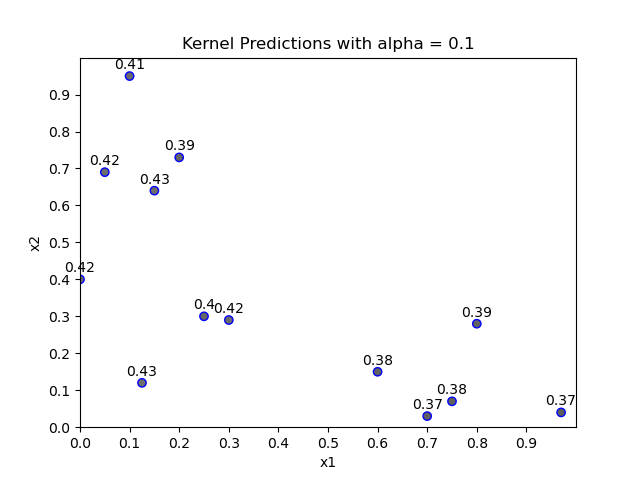
\includegraphics[width=1.1\linewidth]{figures/alpha0.1.png}
  \caption{Alpha Value 0.1}
  \label{fig:sub1}
\end{subfigure}%
\begin{subfigure}{0.33\textwidth}
  \centering
  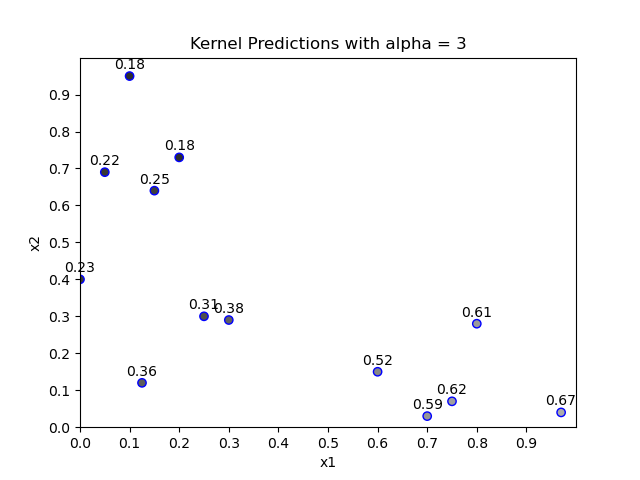
\includegraphics[width=1.1\linewidth]{figures/alpha3.png}
  \caption{Alpha Value 3}
  \label{fig:sub2}
\end{subfigure}
\begin{subfigure}{0.33\textwidth}
  \centering
  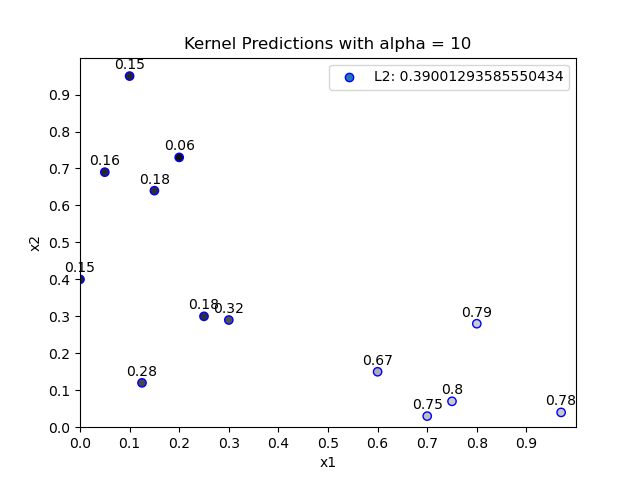
\includegraphics[width=1.1\linewidth]{figures/alpha10.png}
  \caption{Alpha Value 10}
  \label{fig:sub2}
\end{subfigure}
\caption{Kernelized Regression Plots}
\label{fig:test}
\end{figure}


\begin{figure}
\centering
\begin{subfigure}{0.33\textwidth}
  \centering
  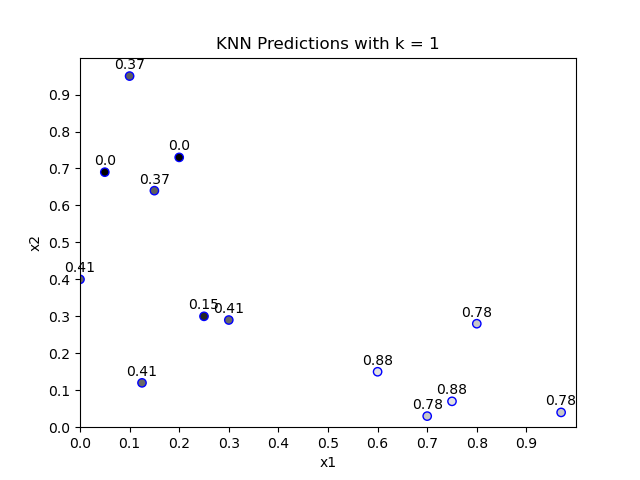
\includegraphics[width=1.1\linewidth]{figures/k1.png}
  \caption{K Value 1}
  \label{fig:sub1}
\end{subfigure}%
\begin{subfigure}{0.33\textwidth}
  \centering
  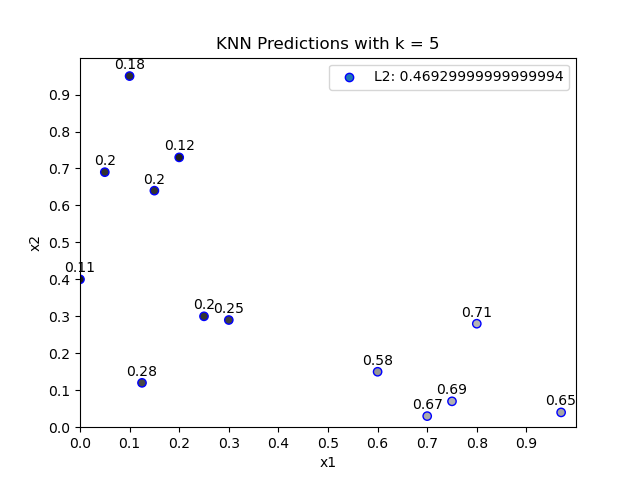
\includegraphics[width=1.1\linewidth]{figures/k5.png}
  \caption{K Value 5}
  \label{fig:sub2}
\end{subfigure}
\begin{subfigure}{0.33\textwidth}
  \centering
  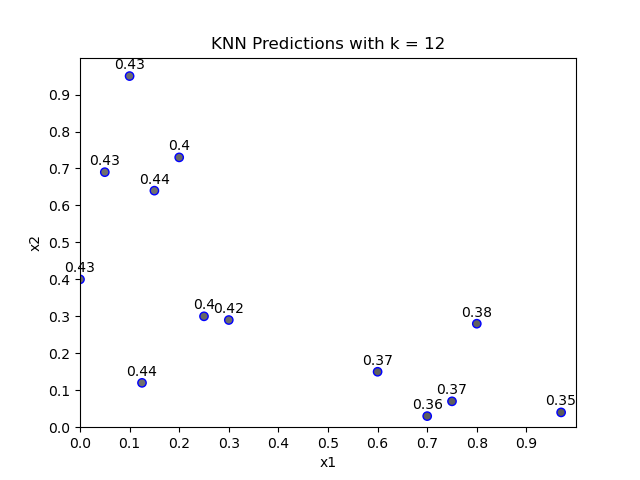
\includegraphics[width=1.1\linewidth]{figures/k12.png}
  \caption{K Value 12}
  \label{fig:sub2}
\end{subfigure}
\caption{KNN Regression Plots}
\label{fig:test}
\end{figure}

\begin{tcolorbox}[breakable]

\textbf{(1)}\\

Plots are located above for reference, the remaining code is in the T1P2.py file.\\

\textbf{(2)}\\

The plot with an alpha value of 0.1 appears to be very similar to a KNN plot of $(N -1)NN$ and the plot with an alpha of 10 seems very similar to a plot of 1NN.\\\\
To understand this effect we must consider the effect of alpha on the distance calculation scaling and in turn the kernel function's penalty and weighting for those points. Consider the following equation:

\begin{equation}
\begin{bmatrix}
  x_1 & x_2
 \end{bmatrix}
 \begin{bmatrix}
  \alpha & 0 \\
  0 & \alpha 
 \end{bmatrix}  
 \begin{bmatrix}
  x_1 \\
  x_2 
 \end{bmatrix} = 
  \alpha^2 x_1 + \alpha^2 x_2
\end{equation}

Here you can see that as the $\alpha$ value increases, so does the value of the scale which means that the kernel function's output $\frac{1}{e^{val}}$ will decrease in magnitude as the value grows, hence creating a sort of localization effect such that when the value of alpha increases, so does the localization and when the value of alpha decreases, more points are weighted higher because they are penalized less for their distance from the point being predicted for.\\

What this implies is that when the alpha value is low, localization is lower too, which means more of the points have a greater weight the final prediction of that point such that it seems that we are almost averaging over the whole data-set, where on the other hand if the alpha value is higher then we end up with hyper-localization where we are essentially picking the closest surrounding point.

\end{tcolorbox}

\begin{figure}
\centering
\includegraphics[width=0.4\linewidth]{figures/gradient_alpha_local.png}
\caption{Localization Effect of Alpha}
\label{fig:test}
\end{figure}

\begin{tcolorbox}[breakable]

\textbf{(3)}\\

Let us choose 1NN for our KNN regression. The edge case we want to exploit is how the methods differ when the Mahalanobis Function comes up with the same distance for some number points and some points are equally weighted to be used for prediction. Without loss of generality suppose let us consider that we have 3 non-zero points in our data set such that $a = (x_1, y_1)$,  $b = (x_2, y_2)$ and $c = (x_3, y_3)$ where a, b, and c have the same Mahalalobis distance from each other. Now suppose we are using our regression method to generate $\hat{y}_1$. For 1NN, the predicted value will have to be a single point selected either from b or c, where based on the sorting algorithm of the distances, the choice is likely to be random. Now consider the kernel function, for the function, both b and c have the same distance away from point a and therefore the same penalty, regardless of the alpha, both points will be weighted equally towards the value of a, such that $(y_2 + y_3)/2$ will be the predicted value, and by definition, that value will always be different from $y_3$ or $y_2$ so long as a, b and c are not the same point. In a numerical example, consider the value of y for b to be 10 and for c to be 5, then 1NN will give either 5 or 10 and the kernel-regression will give 7.5 regardless of alpha.\\\\

\textbf{(4)}\\

The reason we did not change alpha is because it would not matter in the end. Alpha is a scaling factor for the Mahalanobis distance calculation, but in KNN we sort the points by the distance which means that if we are conducting a monotonic scalar transformation on the distance values, we are not actually changing which order the values will be sequenced in which means that the scaling of the distance by alpha will not change the order and thereby will not change the resulting predictions or loss.




\end{tcolorbox}


\newpage 

%%%%%%%%%%%%%%%%%%%%%%%%%%%%%%%%%%%%%%%%%%%%%
% Problem 3
%%%%%%%%%%%%%%%%%%%%%%%%%%%%%%%%%%%%%%%%%%%%%

\begin{problem}[Deriving Linear Regression, 10pts]

  In class, we noted that the solution for the least squares linear
  regressions ``looked'' like a ratio of covariance and variance
  terms.  In this problem, we will make that connection more explicit.

  Let us assume that our data are tuples of scalars $(x,y)$ that come from
  some distribution $p(x,y)$.  We will consider the process of fitting
  these data with the best linear model possible, that is a linear
  model of the form $\hat{y} = wx$ that minimizes the expected squared
  loss $E_{x,y}[ ( y - \hat{y} )^2 ]$.\\

\noindent \emph{Notes:} The notation $E_{x, y}$ indicates an
expectation taken over the joint distribution $p(x,y)$.  Since $x$ and
$y$ are scalars, $w$ is also a scalar.
  
  \begin{enumerate}

  \item Derive an expression for the optimal $w$, that is, the $w$
    that minimizes the expected squared loss above.  You should leave
    your answer in terms of moments of the data, e.g. terms like
    $E_x[x]$, $E_x[x^2]$, $E_y[y]$, $E_y[y^2]$, $E_{x,y}[xy]$ etc.

\item Provide unbiased and consistent formulas to estimate $E_{x, y}[yx]$
 and $E_x[x^2]$ given observed data $\{(x_n,y_n)\}_{n=1}^N$.

\item In general, moment terms like $E_{x, y}[yx]$, $E_{x, y}[x^2]$,
  etc. can easily be estimated from the data (like you did above).  If
  you substitute in these empirical moments, how does your expression
  for the optimal $w^*$ in this problem compare with the optimal $w^*$
  that we derived in class/Section 2.6 of the cs181-textbook?

\item As discussed in lecture, many common probabilistic linear regression models assume that variables x and y are jointly Gaussian.  Did any of your above derivations rely on the assumption that x and y are jointly Gaussian?  Why or why not?
    
\end{enumerate}

\end{problem}

\begin{tcolorbox}[breakable]

\textbf{(1)}\\

We want a linear model of the form $\hat{y} = wx$. And we want to optimize our weights by finding the weights that minimize the expected squared loss. 

$$ E_{x,y}[(y - \hat{y})^2] $$

$$ E_{x,y}[(y - \hat{y})^2]  =  E_{x,y}[y^2 - 2y\hat{y}  + \hat{y}^2]$$

Let us now substitute in the definition of our linear model $\hat{y} = wx$,

$$ E_{x,y}[y^2 - 2y\hat{y}  + \hat{y}^2] = E_{x,y}[y^2 - 2wxy  + w^2x^2]$$

We can now use the linearity of expectations and the following fact about the marginal distribution that:

$$ E_{xy}[x^2] = E_x[x^2]$$

$$ E_{xy}[y^2] = E_x[y^2]$$

$$ E_{xy}[x^2] = \int_x\int_y f(x,y)x^2 dxdy$$

$$ \int_x\int_y f(x,y)x^2 dxdy = \int_x f(x)x^2 dx = E_{x}[x^2]$$

Therefore we have:

$$ E_{x,y}[y^2 - 2wxy  + w^2x^2] = E_{y}[y^2] - 2wE_{x,y}[xy] + w^2E_{x}[x^2]$$

Now that we have a quadratic formula, we can optimize and find the vertex without taking the derivative by using the formula $\frac{-b}{2a}$.

$$ w^{*} = \frac{-b}{2a} = \frac{2E_{x,y}[xy]}{2E_{x}[x^2]}  = \boxed{ \frac{E_{x,y}[xy]}{E_{x}[x^2]}}$$\\

\textbf{(2)}\\

In order to find unbiased and consistent formulas to estimate the expectations from the data, we can take advantage of the definition of sample expectation. We know that by the Law of Large Numbers the sample mean shall converge to the true mean such that the following formula provides consistency,

$$\lim_{n \to \infty} (\frac{1}{n})\sum\limits_n x_n y_n = xy$$

This implies that the following expression can be reduced by linearity of Expectation,

$$ E[(\frac{1}{n})\sum\limits_n x_n y_n] = \frac{1}{n} \sum_n E(x_n y_n) $$

Knowing that each $x_n y_n$ have i.i.d. and $x_n y_n$ will converge to $x y$ by the Law of Large Numbers, 

$$ \frac{1}{n} \sum_n E(x_n y_n) \to (1/n)*n E(x y) = E(x y) $$

Similarly with $E_{x}[x^2]$, 

$$\lim_{n \to \infty} (\frac{1}{n})\sum\limits_n {x_n}^2 = x^2$$

Where we can apply the linearity of expectations and the symmetry along with the Law of Large Numbers,

$$ E[(\frac{1}{n})\sum\limits_n {x_n}^2] = \frac{1}{n} \sum_n E({x_n}^2) $$

$$ \frac{1}{n} \sum_n E({x_n}^2) \to (1/n)*n E(x^2) = E(x^2) $$

Therefore our estimates for the expectation terms are,

$$ \boxed{E_{x,y}[\bar{x}_n \bar{y}_n] = \left(\frac{1}{n}\right)\sum\limits_n x_n y_n}$$

$$ \boxed{E_{x}[{\bar{x}_n}^2] = \left(\frac{1}{n}\right)\sum\limits_n {x_n}^2}$$\\\\

\textbf{(3)}\\\\

Using our estimate from above, we can substitute it in to our expression to derive the following formula for the estimate of $w^{*}$

$$ \hat{w}^{*} = \frac{\left(\frac{1}{n}\right)\sum\limits_n x_n y_n}{\left(\frac{1}{n}\right)\sum\limits_n {x_n}^2} = \frac{\sum\limits_n x_n y_n}{\sum\limits_n {x_n}^2}$$

In comparison, we have the following equation from section 2.6,

$$ w^{*} = (X^TX)^{-1}X^TY $$

This equation is comparable because $X^TX$ is a 1 by N vector multiplied by a N by 1 vector (NOTE: we are omitting the bias factor here), the result is a 1 by 1 or a scalar value such that the $X^TX$ term is equivalent to:

$$ X^TX = \sum\limits_n {x_n}^2 $$

$$ (X^TX)^{-1} = \frac{1}{\sum\limits_n {x_n}^2} $$

Along the same lines the $X^TY$ term where $X^T$ is 1 by N and Y is N by 1, then the value of the product is also scalar such that that value is comparable to:

$$ X^TY = \sum\limits_n x_n y_n $$

Therefore we have that, 

$$ (X^TX)^{-1}X^TY = w^{*} = \hat{w}^{*} = \frac{\sum\limits_n x_n y_n}{\sum\limits_n {x_n}^2}$$

This relation demonstrates the method of deriving estimates of empirical moments used to optimize the weights in a Statistical approach versus the Linear Algebra approach show the consistency among the various approaches to linear regression as discussed in section 2.6.3 and Lecture 3 (Feb 2.).\\\\

\textbf{(4)}\\

\textit{No}, we did not make an assumption that the variables x and y are jointly Gaussian, in our derivation of the estimate for the weight we used the linearity of expectations and the Law of Large Numbers, along with the definition of the sample mean, none of which are inherently derived from the normal (Gaussian) distribution. Therefore, we do not rely on the assumption that the joint distribution was Gaussian, in fact as discussed in class, there are a variety of different models like student-T, Laplace that can be used as generative models as the the normal distribution was in  section 2.6.3 to come to the same derivation of the $w^{*}$ value, and the conclusion that \textit{minimizing a least squares loss function is equivalent to maximizing the probability under the
assumption of a linear model with Gaussian noise}.



\end{tcolorbox}


%%%%%%%%%%%%%%%%%%%%%%%%%%%%%%%%%%%%%%%%%%%%%
% Problem 4
%%%%%%%%%%%%%%%%%%%%%%%%%%%%%%%%%%%%%%%%%%%%%

\begin{problem}[Modeling Changes in Republicans and Sunspots, 15pts]
  
 The objective of this problem is to learn about linear regression
 with basis functions by modeling the number of Republicans in the
 Senate. The file \verb|data/year-sunspots-republicans.csv| contains the
 data you will use for this problem.  It has three columns.  The first
 one is an integer that indicates the year.  The second is the number
 of Sunspots observed in that year.  The third is the number of Republicans in the Senate for that year.
 The data file looks like this:
 \begin{csv}
Year,Sunspot_Count,Republican_Count
1960,112.3,36
1962,37.6,34
1964,10.2,32
1966,47.0,36
\end{csv}

You can see scatterplots of the data in the figures below.  The horizontal axis is the Year, and the vertical axis is the Number of Republicans and the Number of Sunspots, respectively.

\begin{center}
\includegraphics[width=.5\textwidth]{data/year-republicans}
\end{center}

\begin{center}
\includegraphics[width=.5\textwidth]{data/year-sunspots}
\end{center}

(Data Source: \url{http://www.realclimate.org/data/senators_sunspots.txt})\\
\vspace{-5mm}


\vspace{0.5cm}
\noindent\emph{Make sure to include all required plots in your PDF.}

\begin{enumerate}

\item In this problem you will implement ordinary least squares regression using 4 different basis functions for
\textbf{Year (x-axis)} v. \textbf{Number of Republicans in the Senate (y-axis)}. Some starter Python code
that implements simple linear regression is provided in \verb|T1_P4.py|.

First, plot the data and regression lines for each of the following sets of basis functions, and include
the generated plot as an image in your submission PDF. You will therefore make 4 total plots:
\begin{enumerate}
  \item[(a)] $\phi_j(x) = x^j$ for $j=1, \ldots, 5$\\
    ie, use basis $y = a_1 x^1 + a_2 x^2 + a_3 x^3 + a_4 x^4 + a_5 x^5$ for some constants $\{a_1, ..., a_5\}$. 
    \item[(b)] $\phi_j(x) = \exp{\frac{-(x-\mu_j)^2}{25}}$ for $\mu_j=1960, 1965, 1970, 1975, \ldots 2010$
  \item[(c)] $\phi_j(x) = \cos(x / j)$ for $j=1, \ldots, 5$
  \item[(d)] $\phi_j(x) = \cos(x / j)$ for $j=1, \ldots, 25$
\end{enumerate}
\vspace{-2mm}
{\footnotesize * Note: Be sure to add a bias term for each of the basis functions above.}

Second, for each plot include the residual sum of squares error. Submit the generated plot and residual sum-of-squares error for each basis in your LaTeX write-up.
\end{enumerate}

\end{problem}

\begin{framed}
\noindent\textbf{Problem 4} (cont.)\\
\begin{enumerate}
\setcounter{enumi}{1}
\item Repeat the same exact process as above but for \textbf{Number of Sunspots (x-axis)} v. \textbf{Number of Republicans in the Senate (y-axis)}. 
Now, however, only use data from before 1985, and only use basis functions (a), (c), and (d) -- ignore basis (b). You will therefore make 3 total plots. For each plot make sure to also include the residual sum of squares error.

Which of the three bases (a, c, d) provided the "best" fit? \textbf{Choose one}, and keep in mind the generalizability of the model. 

Given the quality of this fit, do you believe that the number of sunspots controls the number of Republicans in the senate (Yes or No)?
\end{enumerate}
\end{framed}

\textbf{(1)}

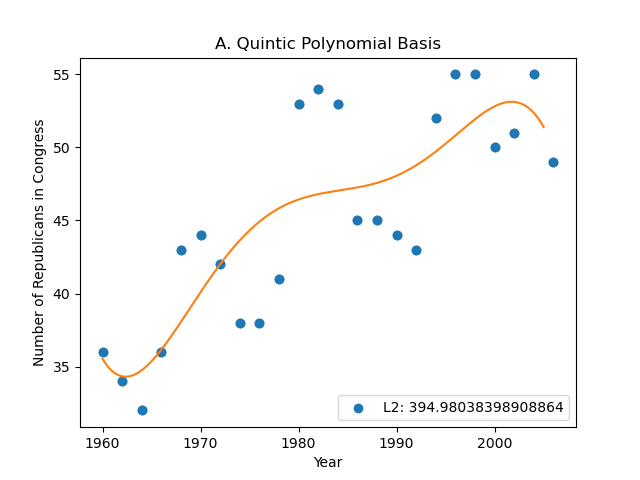
\includegraphics[width=0.7\linewidth]{figures/r1.png}

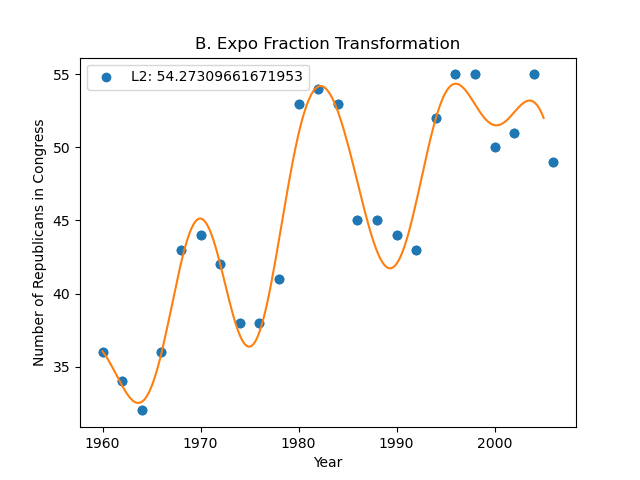
\includegraphics[width=0.7\linewidth]{figures/r2.png}

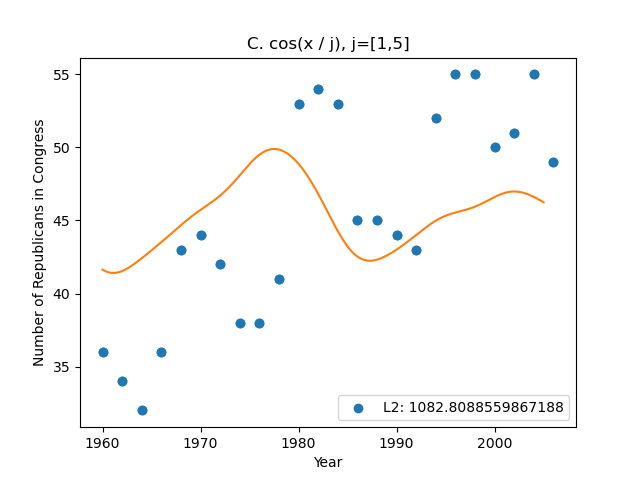
\includegraphics[width=0.7\linewidth]{figures/r3.png}

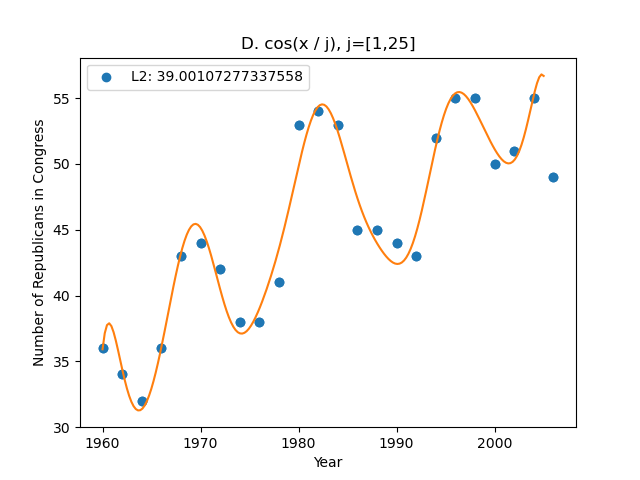
\includegraphics[width=0.7\linewidth]{figures/r4.png}

\textbf{(2)}


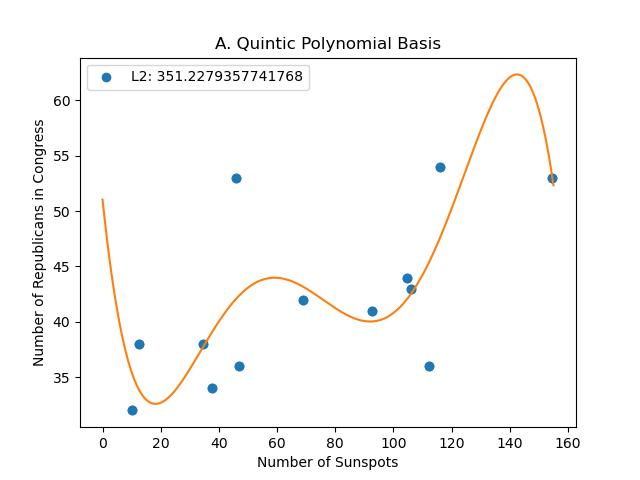
\includegraphics[width=0.7\linewidth]{figures/r5.png}

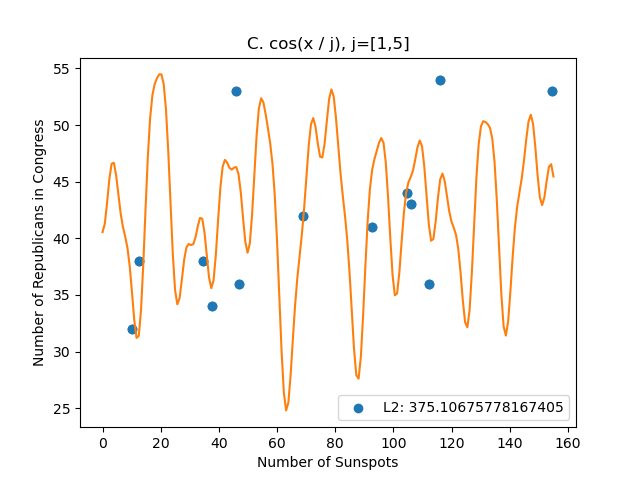
\includegraphics[width=0.7\linewidth]{figures/r7.png}

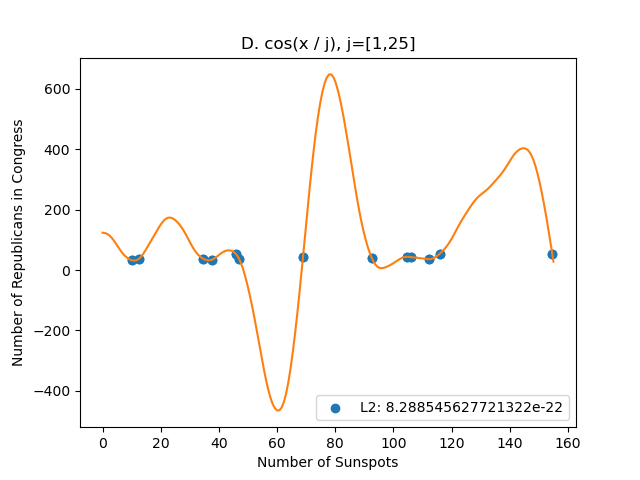
\includegraphics[width=0.7\linewidth]{figures/r8.png}

\begin{tcolorbox}[breakable]

The model with the best fit seems to be the quintic polynomial (Basis A), it seems to be the most generalizable considering the data-set's trend although it doesn't have to lowest loss with a value of 351.22. The C. basis function seems to oscillate wildly and seems to completely miss the data and has the greatest loss with a value of 375.11. The basis function for D. on the order hand seems to over fit the data, where every inflection point is also a data point and has the lowest loss which is effectively zero. However, this over fit means that it most likely does not serve as a good predictor for other data values, at least not as well as the polynomial which captures a somewhat general trend. Yet even considering the basis function for A, the polynomial has a large L2 Loss due to its misfit, and based on that observation it seems that it is unlikely that the number of sunspots predicts the number of republicans in Congress.

\end{tcolorbox}


\newpage
%%%%%%%%%%%%%%%%%%%%%%%%%%%%%%%%%%%%%%%%%%%%%
% Name and Calibration
%%%%%%%%%%%%%%%%%%%%%%%%%%%%%%%%%%%%%%%%%%%%%
\subsection*{Name}

\subsection*{Collaborators and Resources}
Whom did you work with, and did you use any resources beyond cs181-textbook and your notes?\\\\

Viet Vu, Jonathan Lu

\subsection*{Calibration}
Approximately how long did this homework take you to complete (in hours)? 

18 hrs.

\end{document}




